\subsection{Dilution Factor Calculation}
\label{sec::df}
In the longitudinally polarized deuterated-ammonia (ND$_3$) target, the selected events include contributions from deuterium, nitrogen, helium coolant and target-cell material. It is therefore necessary to determine the fraction originating from deuterium. This fraction is referred to as the dilution factor, $D_f$. The RGC dilution-factor formalism is described in the standalone document ``\href{https://clasweb.jlab.org/wiki/images/7/72/Dilution_Factor_Determination_for_RG_C_10-16-26.pdf}{Dilution Factor Determination for RG-C}'' by S.~E.~Kuhn, D.~Holmberg and D.~W.~Upton. We calculate $D_f$ directly from charge-normalized ND$_3$, C, CD$_2$, He-bath and empty-target measurements, using Eq.~7 and the ND$_3$ coefficients in Table~II of that document.

The auxiliary-target measurements separate the carbon-like nuclear contribution, helium and cell material from the deuterium contribution. The calculation also accounts for the helium displaced by the solid targets. All samples receive the same exclusivity cuts as the ND$_3$ data from their run period. With $n_T=N_T/Q_T$, the thermally corrected expression is
\begin{align}
S &= n_{\mathrm{CD}_2}-0.765506n_C-0.000757116n_{\mathrm{He}}-0.233737n_{\mathrm{ET}},\\
D &= n_{\mathrm{CD}_2}-0.170112n_C-0.863533n_{\mathrm{He}}+0.0336457n_{\mathrm{ET}},\\
D_f &= \frac{(n_{\mathrm{ND}_3}-n_{\mathrm{He}})S}{n_{\mathrm{ND}_3}D}.
\end{align}
CD$_2$ was measured only in Sp23. For Su22 and Fa22 we multiply the charge-normalized CH$_2$ yield by the Sp23 CD$_2$/CH$_2$ ratio, determined in the same kinematic bin. Figure~\ref{fig:df_controls} compares the measured Sp23 distributions.

\begin{figure}[htbp]\centering
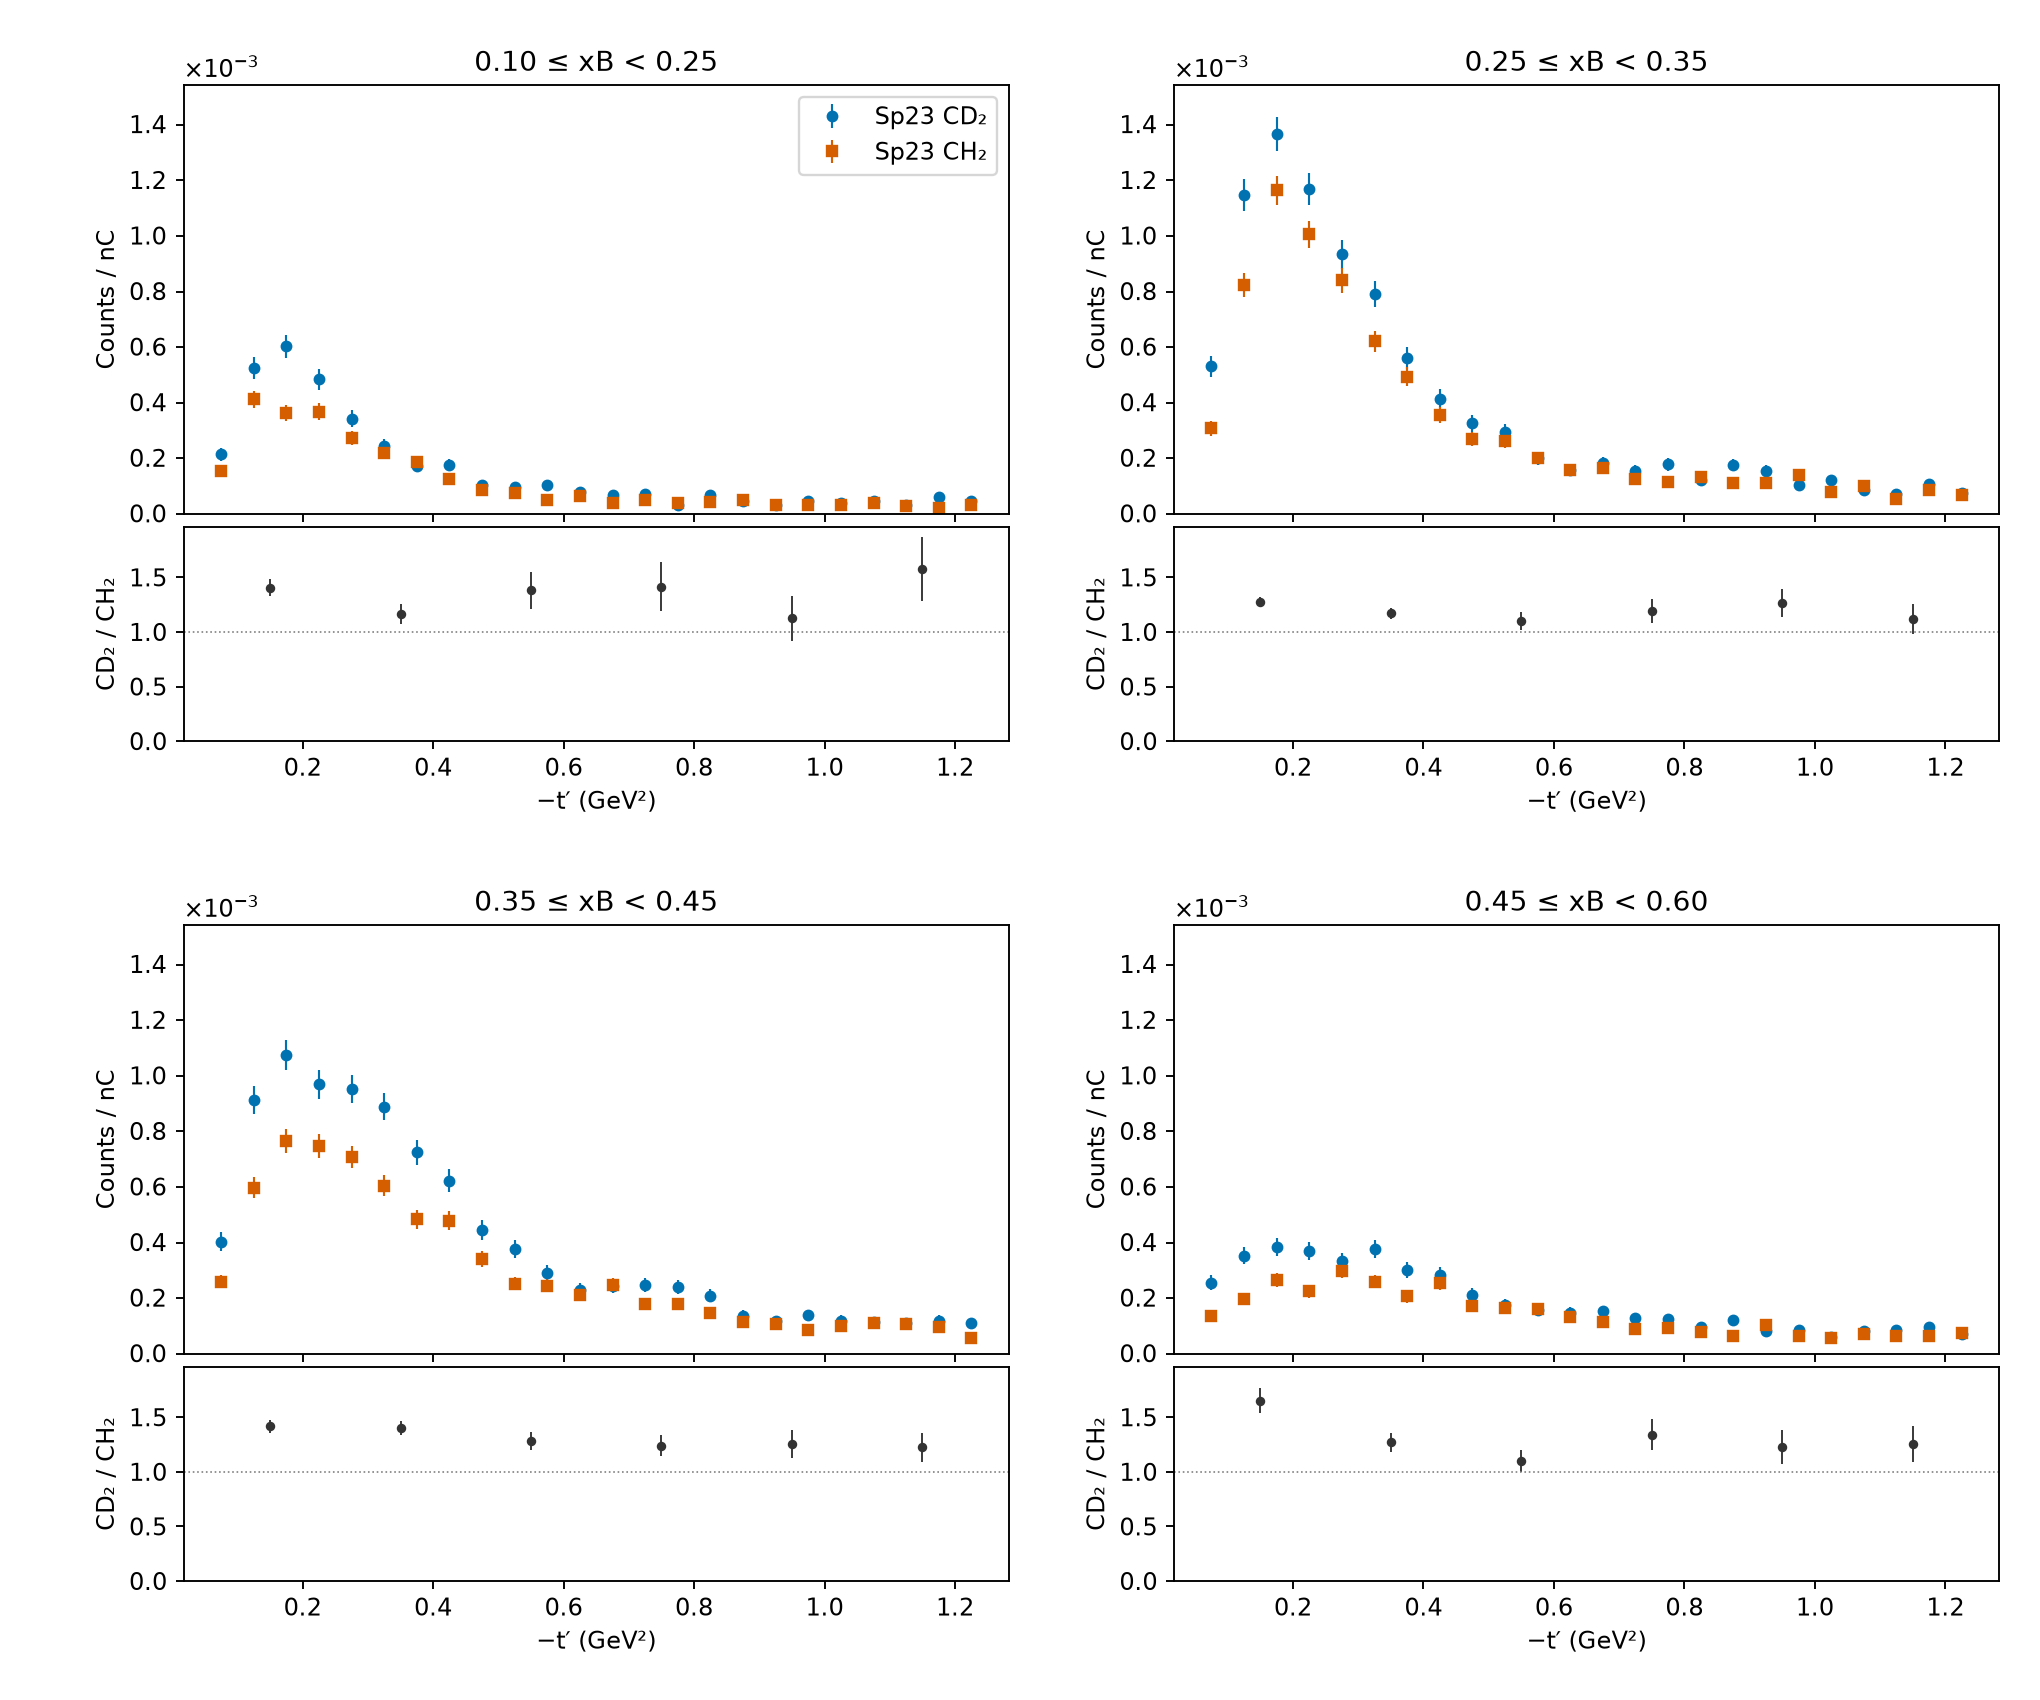
\includegraphics[width=\linewidth]{figures/asymmetry_extraction/dilution_factor/cd2_ch2_distributions.png}
\caption{Sp23 CD$_2$ and CH$_2$ yields normalized to charge, with their ratios below. The ratio panels use the six analysis bins in $-t'$.}\label{fig:df_controls}
\end{figure}

We first compare the three periods after integrating over either $-t'$ or $x_B$ (Fig.~\ref{fig:df_periods}). Correlated statistical comparisons give $\chi^2/\mathrm{ndf}=9.73/8$ ($p=0.285$) for the $x_B$ dependence and $6.43/12$ ($p=0.893$) for the $-t'$ dependence. The comparisons include correlations from the shared Sp23 measurements.

\begin{figure}[htbp]\centering
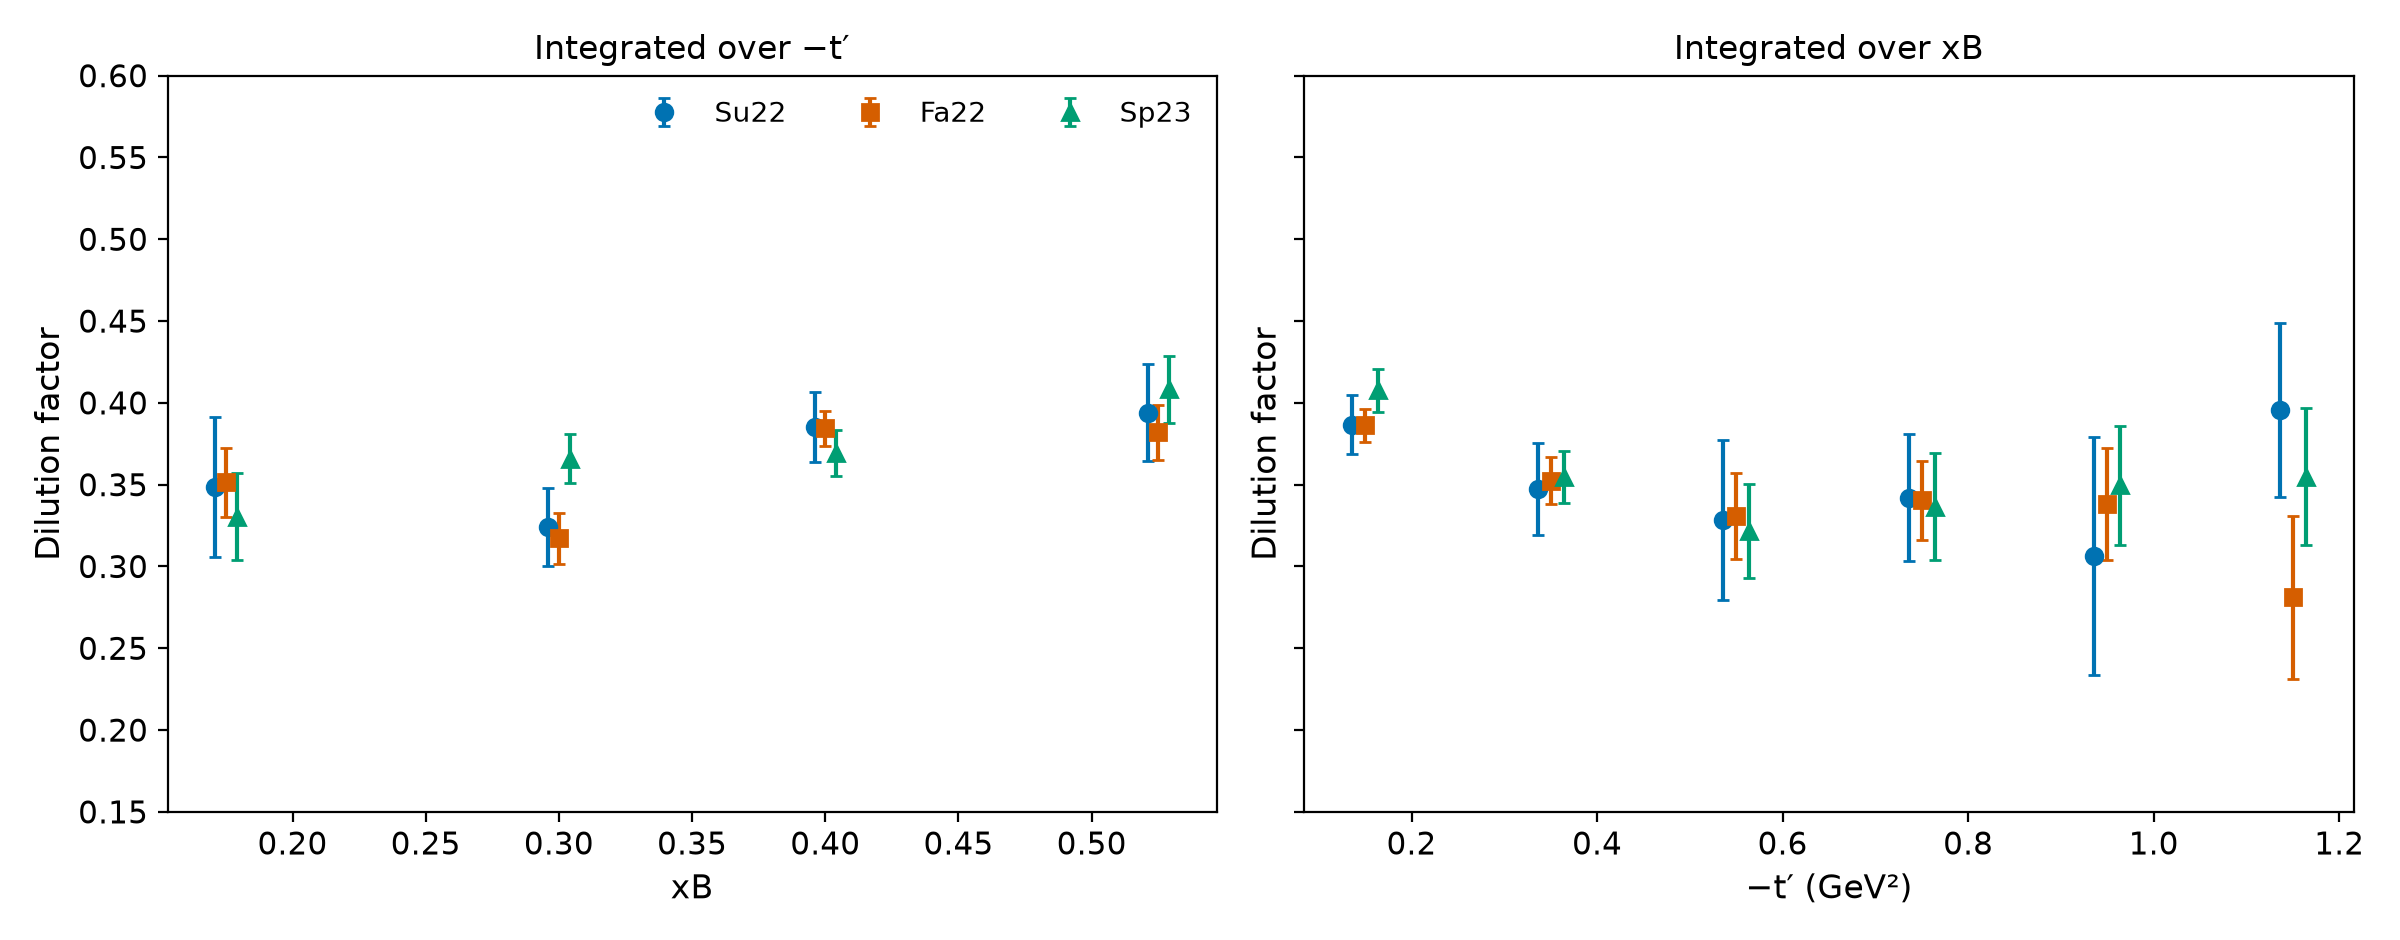
\includegraphics[width=\linewidth]{figures/asymmetry_extraction/dilution_factor/period_agreement.png}
\caption{Period comparisons integrated over $-t'$ (left) or $x_B$ (right). Error bars show statistical standard deviations from Poisson replicas. Points are slightly displaced horizontally for readability.}\label{fig:df_periods}
\end{figure}

For the released target-spin ratios, adjacent fine bins are merged before the material calculation. A shared-period dilution factor is fitted in each of the twelve merged bins, retaining independent period target rates and the common Sp23 CD$_2$/CH$_2$ transfer. Statistical errors are the standard deviations of 2,000 independent Poisson-replica fits per bin. The $LU$ ratio receives no direct dilution correction. The earlier 24-bin corrections remain available as a cross-check but are not used for the released three-bin $UL$ ratios.
\clearpage
\begin{longtable}{rrrr}
\caption{Shared-period dilution factors in the twelve target-sector bins.}\\
\toprule Bin & $D_f$ & Statistical error & Joint deviance\\\midrule\endhead
1 & 0.3346 & 0.0239 & 0.74\\
2 & 0.3915 & 0.0476 & 5.42\\
3 & 0.3108 & 0.0632 & 2.06\\
4 & 0.3423 & 0.0126 & 6.53\\
5 & 0.3233 & 0.0277 & 4.47\\
6 & 0.3230 & 0.0381 & 0.02\\
7 & 0.4000 & 0.0102 & 1.21\\
8 & 0.3433 & 0.0247 & 1.09\\
9 & 0.3282 & 0.0351 & 1.46\\
10 & 0.4378 & 0.0141 & 3.54\\
11 & 0.3107 & 0.0409 & 0.15\\
12 & 0.3367 & 0.0461 & 0.66\\
\bottomrule\end{longtable}

\begin{figure}[p]\centering
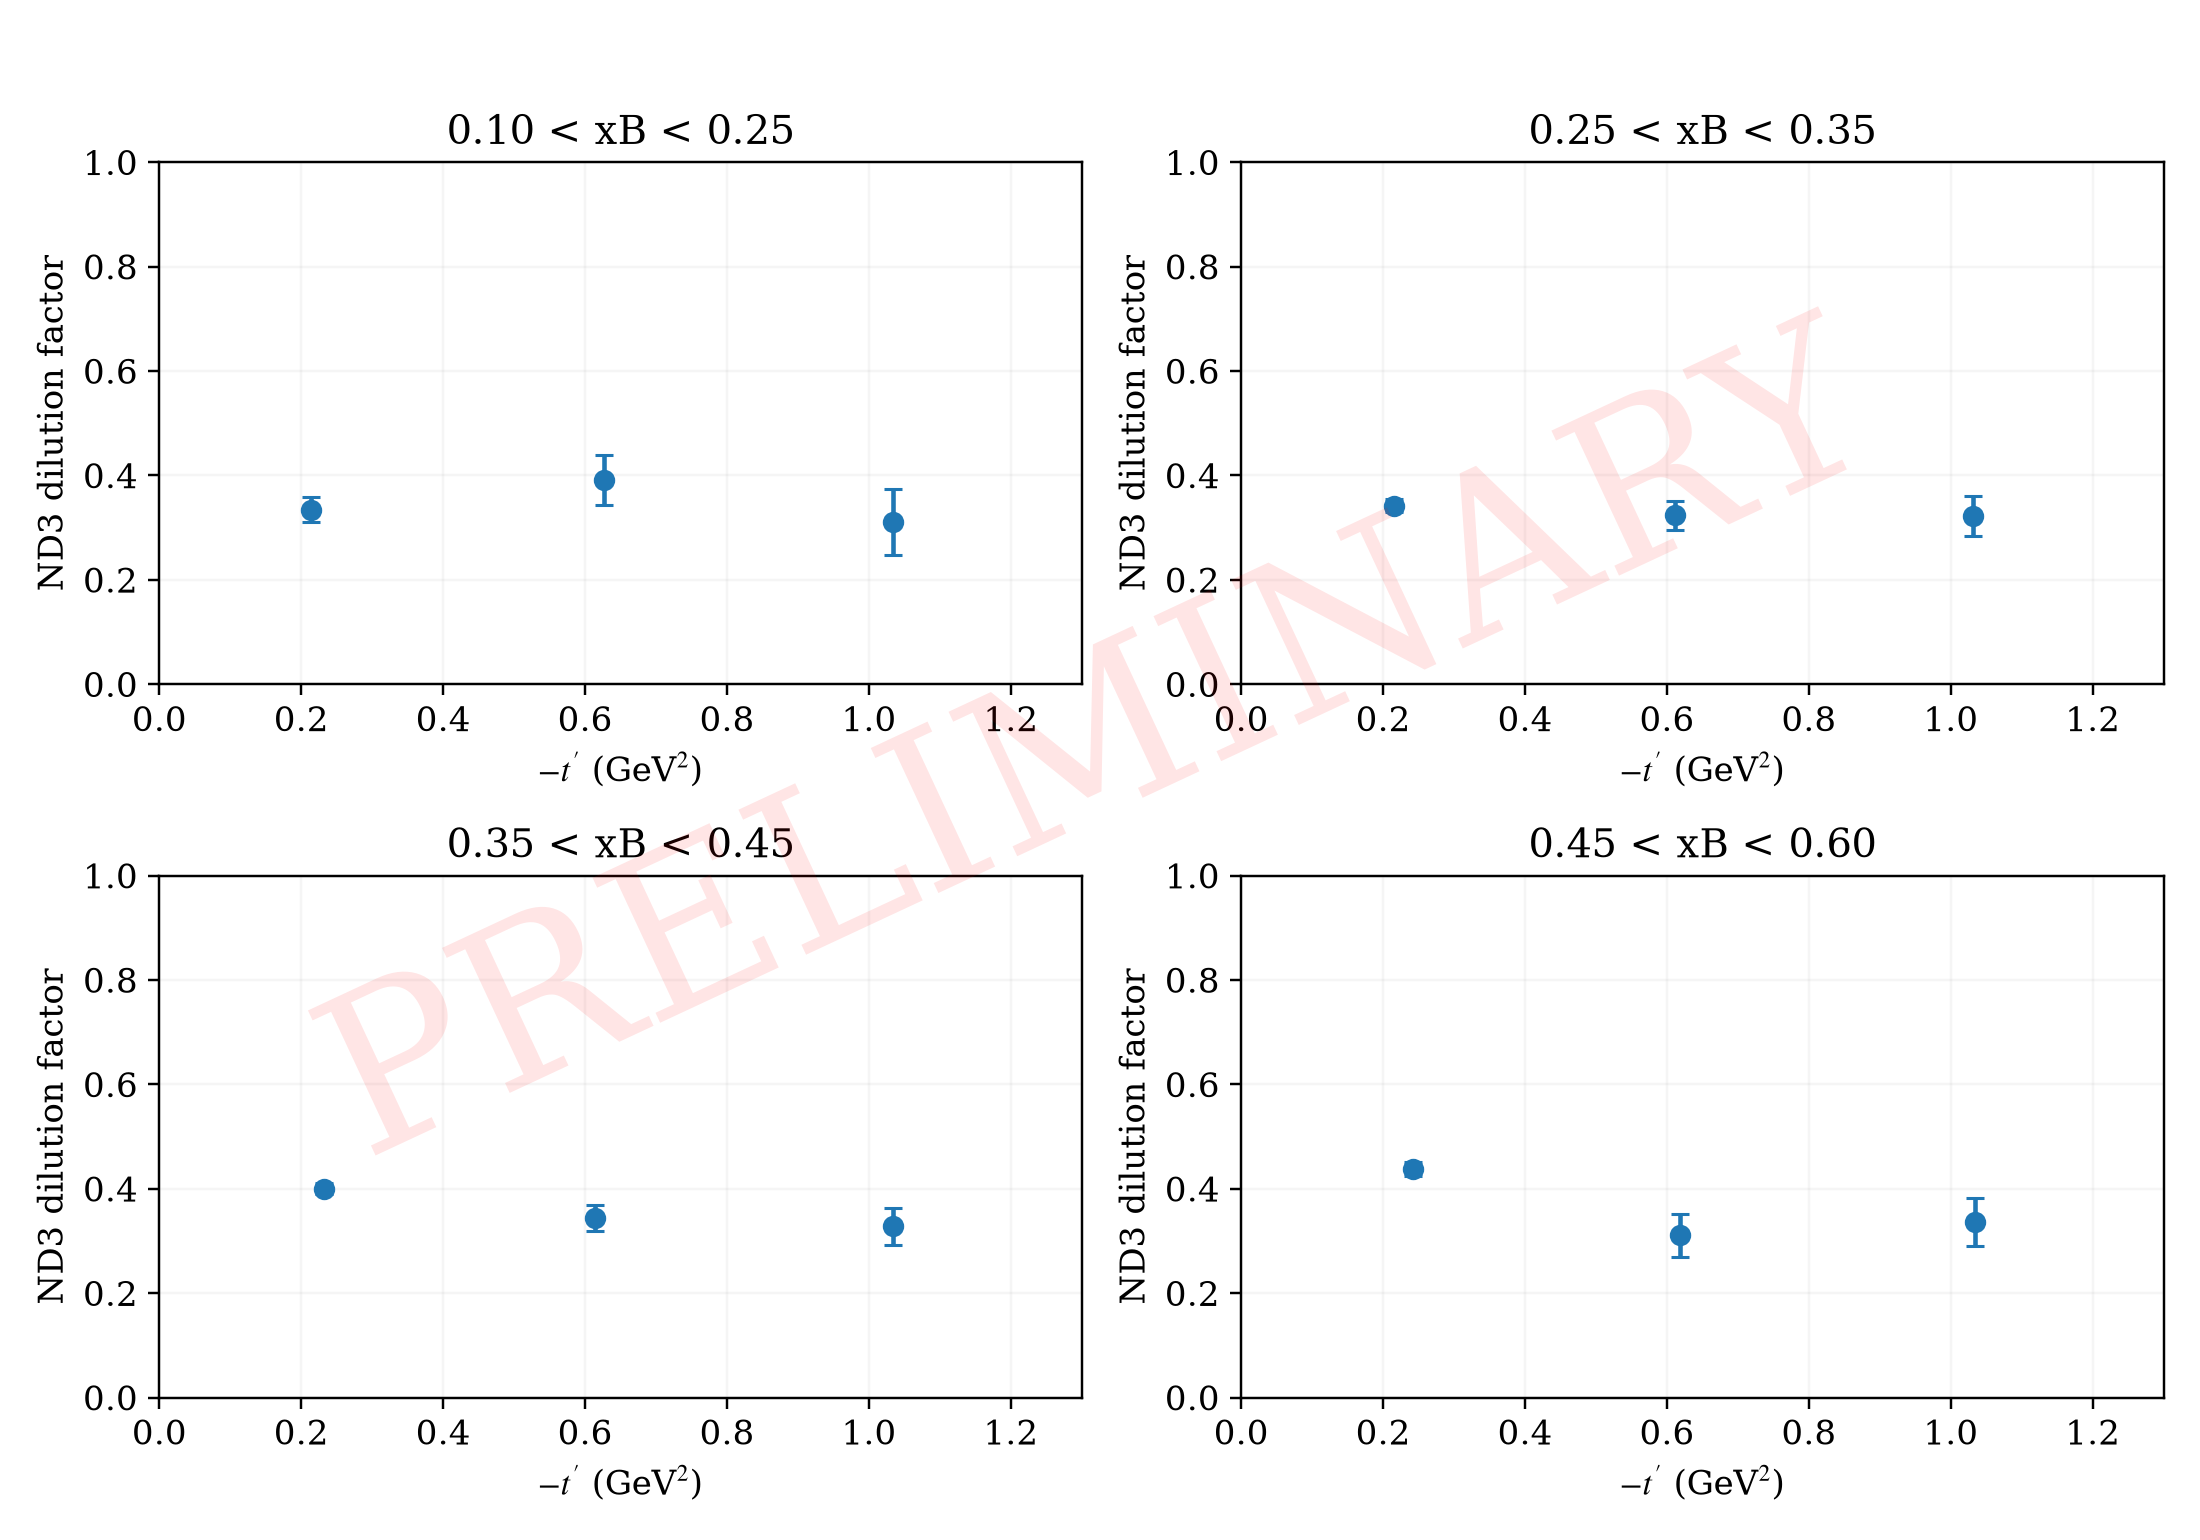
\includegraphics[width=\linewidth]{figures/results/dilution_12_bins.png}
\caption{Shared-period dilution factors in the twelve target-sector bins. Errors are the standard deviations from 2,000 Poisson-replica fits.}\label{fig:release_dilution}
\end{figure}
\clearpage
